%!TEX root = ../thesis.tex

\section{背景}
近年,自律移動ロボットは幅広い産業分野で需要が高まっており屋外で雨天においても自律移動できることが望まれている.
しかし,雨天環境での自律移動はLiDARが雨粒を検出し停止,回避動作を行うことにより困難である.
本研究室では,2D LiDARを搭載した屋外自律移動ロボットを研究・開発している.
雨天時の自律移動に関連する研究では雨粒を模擬または,実環境で行っている.
先行研究\cite{mura}では噴霧器で雨天を模擬した環境と雨天環境の比較を行ったが実際の雨天を十分に再現することはできなかった.
そのため,様々な雨量の環境をシミュレートできるシステムが望まれていると考え,雨天時の2DLiDARデータのモデル化を行った.

\section{目的}
本研究は先行研究\cite{mura}を発展させ,新たに解析及びモデル化を行い,2DLiDARが検出する雨をシミュレータ上で再現することを目的とする.

\section{先行研究}
村林\cite{mura}は,2D LiDARが検出する雨をシミュレータ上で再現し,ロボットの自律移動を検証できるシステムを構築するため,雨天時の2D LiDARデータの取得,解析,モデル化を行った.
コンピュータ内で雨天シミュレータを構築するためには,解析内容として「検出された雨粒の距離の分布」「検出された雨粒の時間間隔の分布」「隣り合うレーザで検出された雨粒の距離の分布」のモデル化が必要であると述べている.
これにより,22件の雨天時の2D LiDARデータの取得,「検出された雨粒の距離の分布」「隣り合うレーザで検出された雨粒の距離の分布」を正規近似し,求められた平均距離と標準偏差を一次近似によりモデル化した.

\begin{figure}[h]
  \centering
  \includegraphics[keepaspectratio, scale=0.08]{images/png/rain_robot_wall2.png}
  \caption{2D LiDAR data acquisition experiment in rainy weather (sourse:\cite{mura})}
  \label{Fig:1.1}
\end{figure}

\begin{figure}[h]
  \centering
  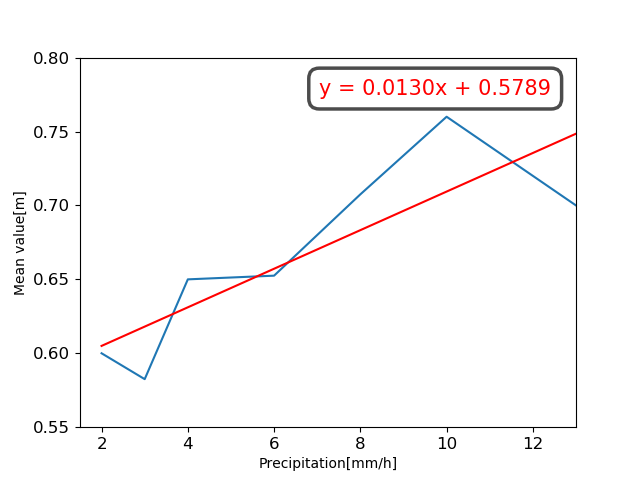
\includegraphics[keepaspectratio, scale=0.38]{images/png/4_3mean_kinji.png}
  \caption{Relationship between the amount of precipitation and the average distance over which the same raindrop was detected (sourse:\cite{mura})}
  \label{Fig:1.2}
\end{figure}

\begin{figure}[h]
  \centering
  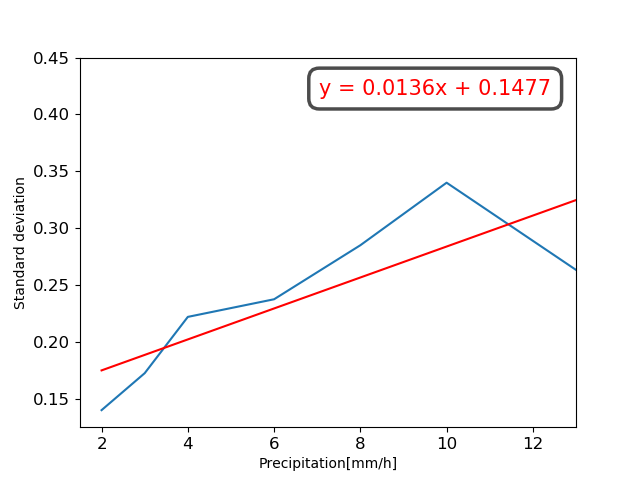
\includegraphics[keepaspectratio, scale=0.38]{images/png/4_3std_kinji.png}
  \caption{Relationship between the amount of precipitation and the standard deviation of the distance over which the same raindrops are detected (sourse:\cite{mura})}
  \label{Fig:1.3}
\end{figure}


\newpage
\section{論文の構成}
本論文は以下のように構築される.第1章では,本研究の背景,目的,先行研究を述べる.
第2章では,本研究に関連する要素技術を述べる.
第3章では,雨天時の2DLiDARデータの追加取得実験について目的,実験装置,方法,結果について述べる.
第4章では,検出された雨粒の時間間隔のモデル化について近似手法,結果,考察を述べる.
第5章では,解析,モデル化したデータを基に開発した雨天シミュレータについて結果と考察を述べる.
第6章では,本論文の結論と今後の展望を述べる.

